\section{Detecting SSH Brute Forcing with Zeek}
Zeek is a powerful network traffic analyzer that plays a crucial role in cybersecurity defenses by monitoring and analyzing network traffic in real time. It's particularly adept at identifying and mitigating security threats, such as SSH brute force attacks. An SSH brute force attack involves an attacker attempting numerous passwords or passphrase combinations to gain unauthorized access to a system. Zeek's approach to detecting such attacks hinges on its ability to scrutinize the intricacies of SSH traffic, focusing on the authentication process.

\subsection{How It Works}
Here's a concise breakdown of how Zeek detects SSH brute forcing:

\begin{enumerate}
    \item \textbf{Monitoring SSH Traffic:} Zeek listens to network traffic, focusing on the SSH protocol to capture the initial handshake, authentication attempts, and the session's lifecycle.
    \item \textbf{Analyzing Authentication Responses:} It examines the size of the server's response packets post-authentication attempts. A response size around 5k bytes often signifies a successful login, which Zeek uses as a heuristic measure.
    \item \textbf{Setting Detection Thresholds:} Parameters like ``password\_guesses\_limit'' and ``guessing\_timeout'' within Zeek's SSH brute forcing script help define the acceptable number of failed login attempts within a certain timeframe, beyond which an attack is presumed.
    \item \textbf{Identifying Brute Force Patterns:} Zeek flags a sequence of failed logins (indicated by ``auth\_success'' set to ``F'') exceeding the predefined threshold within the set timeframe as a brute force attempt.
    \item \textbf{Logging and Alerting:} Following the detection of a brute force attack, Zeek logs the event and can generate alerts, facilitating prompt investigation and response.
\end{enumerate}

\subsection{Detect-bruteforcing.zeek Script:}



\begin{lstlisting}[language=Python, caption=detect-bruteforcing.zeek]
##! Detect hosts which are doing password guessing attacks and/or password
##! bruteforcing over SSH.

@load base/protocols/ssh
@load base/frameworks/sumstats
@load base/frameworks/notice
@load base/frameworks/intel
module SSH;
export {
	redef enum Notice::Type += {
		## Indicates that a host has been identified as crossing the
		## :zeek:id:`SSH::password_guesses_limit` threshold with
		## failed logins.
		Password_Guessing,
		## Indicates that a host previously identified as a "password
		## guesser" has now had a successful login
		## attempt. This is not currently implemented.
		Login_By_Password_Guesser,
	};

	redef enum Intel::Where += {
		## An indicator of the login for the intel framework.
		SSH::SUCCESSFUL_LOGIN,
	};

	## The number of failed SSH connections before a host is designated as
	## guessing passwords.
	const password_guesses_limit: double = 30 &redef;

	## The amount of time to remember presumed non-successful logins to
	## build a model of a password guesser.
	const guessing_timeout = 30 mins &redef;

	## This value can be used to exclude hosts or entire networks from being
	## tracked as potential "guessers". The index represents
	## client subnets and the yield value represents server subnets.
	const ignore_guessers: table[subnet] of subnet &redef;
}

event zeek_init()
	{
	local r1: SumStats::Reducer = [$stream="ssh.login.failure", $apply=set(SumStats::SUM, SumStats::SAMPLE), $num_samples=5];
	SumStats::create([$name="detect-ssh-bruteforcing",
	                  $epoch=guessing_timeout,
	                  $reducers=set(r1),
	                  $threshold_val(key: SumStats::Key, result: SumStats::Result) =
	                  	{
	                  	return result["ssh.login.failure"]$sum;
	                  	},
	                  $threshold=password_guesses_limit,
	                  $threshold_crossed(key: SumStats::Key, result: SumStats::Result) =
	                  	{
	                  	local r = result["ssh.login.failure"];
	                  	local sub_msg = fmt("Sampled servers: ");
	                  	local samples = r$samples;
	                  	for ( i in samples )
	                  		{
	                  		if ( samples[i]?$str )
	                  			sub_msg = fmt("%s%s %s", sub_msg, i==0 ? "":",", samples[i]$str);
	                  		}
	                  	# Generate the notice.
	                  	NOTICE([$note=Password_Guessing,
	                  	        $msg=fmt("%s appears to be guessing SSH passwords (seen in %d connections).", key$host, r$num),
	                  	        $sub=sub_msg,
	                  	        $src=key$host,
	                  	        $identifier=cat(key$host)]);
	                  	}]);
	}

event ssh_auth_successful(c: connection, auth_method_none: bool)
	{
	local id = c$id;

	Intel::seen([$host=id$orig_h,
	             $conn=c,
	             $where=SSH::SUCCESSFUL_LOGIN]);
	}

event ssh_auth_failed(c: connection)
	{
	local id = c$id;

	# Add data to the FAILED_LOGIN metric unless this connection should
	# be ignored.
	if ( ! (id$orig_h in ignore_guessers &&
	        id$resp_h in ignore_guessers[id$orig_h]) )
		SumStats::observe("ssh.login.failure", [$host=id$orig_h], [$str=cat(id$resp_h)]);
	}

\end{lstlisting}


\subsection{Detect-bruteforcing.zeek Script Explanation}
\begin{enumerate}
    \item \textbf{Notice Types Extension} (Lines 10-19): Extends Zeek's notice framework with `Password\_Guessing` and `Login\_By\_Password\_Guesser` for flagging SSH brute force activities and successful logins by flagged hosts.
    
    \item \textbf{Intel Framework Extension} (Lines 21-24): Adds `SSH::SUCCESSFUL\_LOGIN` to the Intel framework, tracking successful SSH logins from hosts involved in brute force activities.
    
    \item \textbf{Configuration Constants} (Lines 26-36): Sets `password\_guesses\_limit` to 30 and `guessing\_timeout` to 30 minutes, defining the threshold for failed login attempts and the time window for their evaluation.
    
    \item \textbf{SumStats Framework Integration} (Lines 38-68): Utilizes `SumStats` for aggregating failed SSH login attempts, employing a reducer with `"ssh.login.failure"` and configuring aggregation functions with a sample size of 5. Threshold evaluation and crossing logic are based on the sum of failed login attempts.
    
    \item \textbf{Successful Login Intel Reporting} (Lines 70-77): Logs successful SSH authentications through the `ssh\_auth\_successful` event using `Intel::seen`, marking with `SSH::SUCCESSFUL\_LOGIN`.
    
    \item \textbf{Failed Login Data Collection} (Lines 79-87): Captures and logs each failed SSH login attempt in the `ssh\_auth\_failed` event, excluding those from `ignore\_guessers`, contributing to brute force detection analysis.
\end{enumerate}
\subsection{SSHAttack Script :}
\begin{lstlisting}[language=Python, caption=sshAttack.zeek]
module SShAttacks;

@load protocols/ssh/detect-bruteforcing
redef SSH::password_guesses_limit=3;

hook Notice::policy(n: Notice::Info) {
  if ( n$note == SSH::Password_Guessing ) {
    add n$actions[Notice::ACTION_LOG];
  }
}

\end{lstlisting}

\subsection{SSHAttack Script Explanation}

\begin{enumerate}
    \item \textbf{Module Declaration}  (Line 1): Declares a new module \texttt{SShAttacks} for organizing script functionalities. The script's module naming might contain a capitalization typo in "SSH".
    \item \textbf{Load Statement}   (Line 3): Instructs Zeek to load the \texttt{detect-bruteforcing} script from the SSH protocol analysis suite, which contains logic for identifying potential brute force attempts.
    \item \textbf{Variable Redefinition}   (Line 4): Sets the brute force detection threshold at three failed attempts by redefining \texttt{SSH::password\_guesses\_limit} to 3.
    \item \textbf{Notice Framework Hook} (Line 6): Implements a hook into Zeek's Notice framework with \texttt{hook Notice::policy(n: Notice::Info) \{ ...\}}, allowing customized handling of notable events, particularly SSH password guessing.
    \item \textbf{Notice Handling}   (Lines 7-8): Within the hook, the script checks for notices related to SSH password guessing (\texttt{n\$note == SSH::Password\_Guessing}) and logs these events (\texttt{add n\$actions[Notice::ACTION\_LOG];}) for further analysis.
\end{enumerate}

\subsection{Simulation : }
Here is the link to PCAP file:
\href{https://www.malware-traffic-analysis.net/tutorials/index.html}{malware-traffic-analysis}\\\\
\begin{itemize}
    \item The PCAP file is executed within Zeek using the 'ssAttack.zeek' script for analysis.
\end{itemize}
\begin{figure}[H]
    \centering
    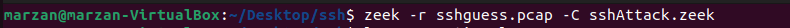
\includegraphics[width=1\linewidth]{images//UDP_reflection/ssh_1.png}
    \caption{Executing PCAP file in Zeek with 'ssAttack.zeek' script}
    \label{fig:enter-label}
\end{figure}

\begin{itemize}
    \item This notice log entry from Zeek indicates that the IP address 192.168.56.1 was detected attempting SSH password guessing, observed over three connections to 192.168.56.103. The activity triggered a SSH::Password\_Guessing alert, and the system took the action to log the event (Notice::ACTION\_LOG). An alert suppression period of one hour (3600.000000 seconds) was set following this detection.
\end{itemize}
\begin{figure}[H]
    \centering
    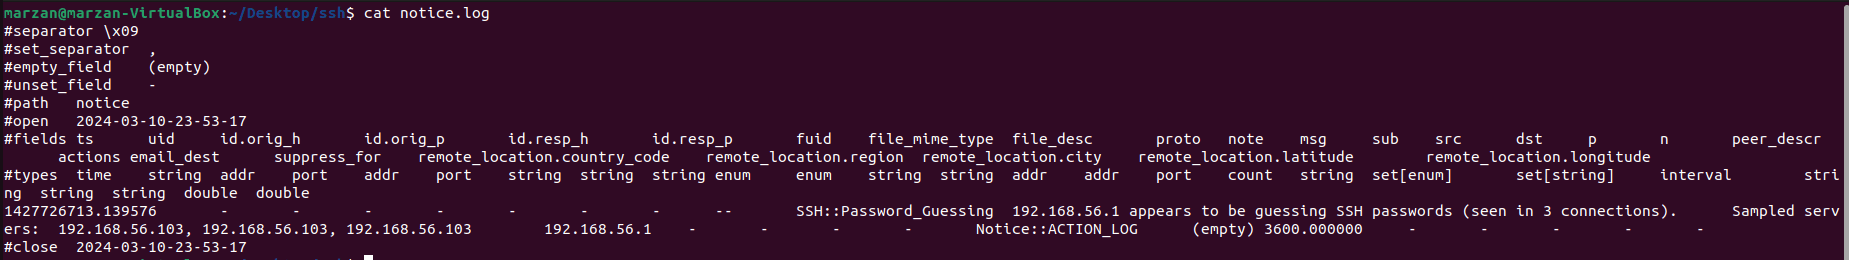
\includegraphics[width=1\linewidth]{images//UDP_reflection/ssh_2.png}
    \caption{notice.log}
    \label{fig:enter-label}
\end{figure}

\begin{itemize}
    \item In BRIM, the notice log entry is presented in a structured tabular format, detailing the detection of an SSH password guessing attempt.
\end{itemize}
\begin{figure}[H]
    \centering
    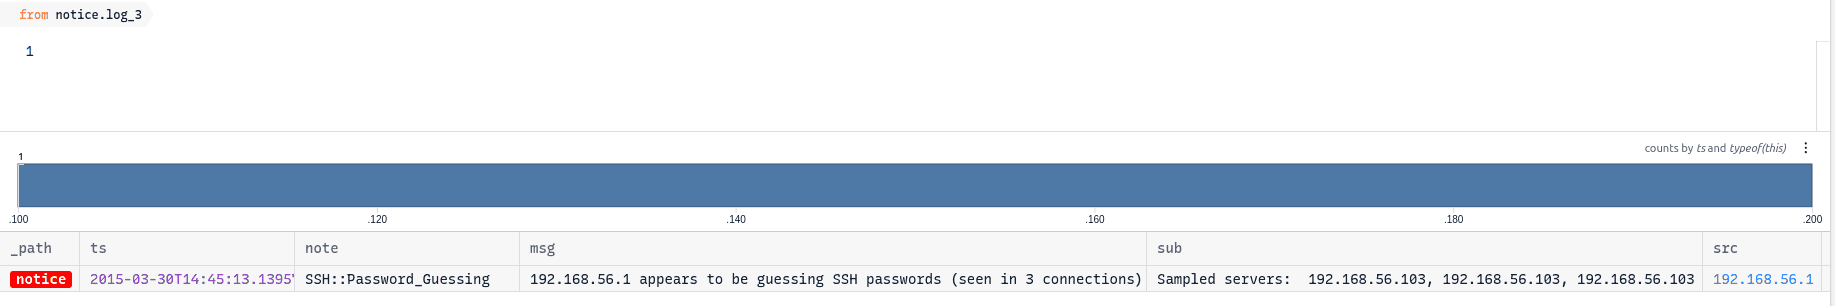
\includegraphics[width=1\linewidth]{images//UDP_reflection/ssh_3.png}
    \caption{notice.log in BRIM}
    \label{fig:enter-label}
\end{figure}


